\chapter{Versuch}
In dem Versuch soll getestet werden, ob der Nutzen von Trackern die Performanz und das Embodiment eines Nutzers gegenüber einer Inverse-Kinematik Lösung für Avatare erhöht. Es wurden zwei Gruppen getestet, die miteinander verglichen werden. Eine Gruppe durchläuft das Experiment mit einem durch IK animierten Avatar. Der Avatar der anderen Gruppe wird mithilfe von sechs zusätzlichen Trackern durch die Bewegungen der Testperson animiert. 
Der Versuchsaufbau in Form eines Ausweichspiels ist für beide Gruppen identisch. Alle Probanden müssen roten Objekten ausweichen während sie grüne Objekte einsammeln sollen. In dem virtuellen Raum befindet sich in Blickrichtung ein großer Spiegel, um den Fokus auf den Avatar zu lenken.
Jedem Teilnehmer wird der gleiche Avatar in Form einer Holzpuppe zur Verfügung gestellt.


\section{Konzeption}
Die Entscheidungen im Versuchsaufbau basieren darauf, den Fokus auf die Animation des Avatars zu legen. Um das zu erreichen werden die Aspekte des Embodiments neben der Agency so gering wie möglich gehalten. Vor allem der Aspekt des Body Ownerships wird vernachlässigt, indem der bereitgestellte Avatar mehr einer Holzpuppe als einem echten Menschen ähnelt. Somit spielen auch unterschiedliche Geschlechter und Hautfarben der Probanden eine kleinere Rolle, da sich niemand perfekt mit dem Avatar identifizieren können sollte. Die Umgebung ist ebenfalls so gestaltet, dass sie möglichst wenig Presence auslöst. So befindet der Teilnehmer sich in einem abstrakten, größtenteils leeren Raum. Der Boden ist mit einer kachelartigen Textur ausgestattet, die bei der Einschätzung von Distanzen helfen soll. Es werden keinerlei Geräusche eingesetzt, da Ton Einfluss auf das Embodiment haben kann und somit die Ergebnisse verfälschen könnte. 
Ein weiteres Element, das den Fokus des Versuchs auf den Avatar und dessen Bewegungen lenkt ist der Spiegel im Raum, der eine Komplette Wand einnimmt. Der Spiegel soll zum einen Helfen, den Fokus auf den Avatar zu lenken. Da dem Teilnehmer keine Zeit während des Spiels gegeben wird, um den Avatar in Ruhe zu untersuchen, bietet der Spiegel die Möglichkeit, während der Konzentration auf die sich bewegenden Objekte, den Avatar zu sehen und wahrzunehmen. Zum anderen soll der Spiegel bei der Einschätzung der Entfernung der Objekte helfen.

^^ nochmal überarbeiten

\begin{figure}[h]
  \makebox[\textwidth]{
    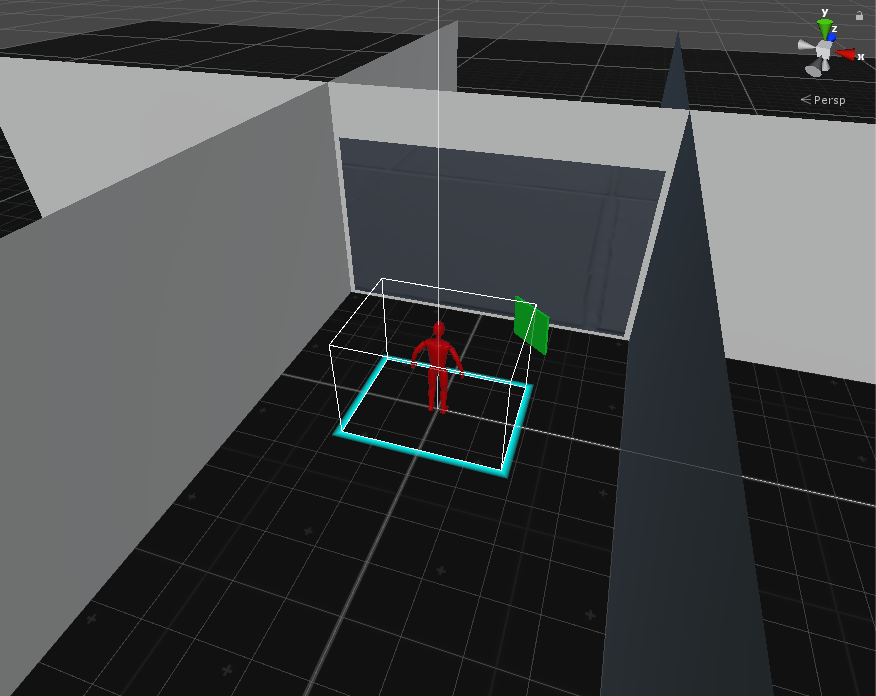
\includegraphics[width=\textwidth]{Bilder/Game/AltesSetup.png}
  }
  \caption[Altes Setup der Anwendung]{Ein früher Prototyp der Anwendung in Unity}
  \label{fig:oldSetup}
\end{figure}

In Abbildung \ref{fig:oldSetup} ist ein früher Prototyp der Anwendung dargestellt. Erst später in der Entwicklungsphase wurde die rote Farbe des Avatars in ein hellbraun umgeändert, da die Farbe zu sehr den Hazards glich.


Der Versuch wurde nach einem Inter-Subjekt Design durchgeführt. Bei Inter-Subjekt Design wird von jedem Probanden jeweils nur eine der Versuchsbedingungen durchgeführt. Dadurch wird vermieden, dass sich die Versuchspersonen zu stark auf den Unterschied zwischen den Versuchsbedingungen konzentrieren und somit die Antworten verfälscht werden könnten. Außerdem könnte bei einem Intra-Subjekt Design, bei dem jeder Proband alle Bedingungen durchläuft, die als zweites durchgeführte Versuchsbedingung fälschlicherweise höhere Embodiment Werte aufweisen, da sich das Gefühl von Embodiment erst nach einer Gewissen Zeit in der Virtuellen Umgebung entwickelt.


\section{Hypothese}
Die Immersion des Systems bei der Versuchsbedingung mit den Trackern ist nach Slaters Definition von Immersion \cite{Slater2003}\cite{Slater1999} höher. Das liegt daran, dass die Tracker dem Benutzer mehr Kontrolle über den Avatar geben und somit mehr Reize stimulieren. Statt drei Kontrollierbaren Punkten im Aufbau ohne Tracker liefert der Aufbau mit Trackern neun Kontrollierbare Punkte und virtualisiert somit mehr Reize des Gehirns.
Aufgrund der erhöhten Immersion mit Trackern wird vermutet, dass das Embodiment durchschnittlich ebenfalls erhöht wird, da Embodiment eine Reaktion auf Immersion ist. Vor allem der Bereich Agency von Embodiment wird in dem Experiment angesprochen, daher sollte der größte messbare Unterschied zwischen den Gruppen in der Kategorie Agency sein.
Die Performanz sollte sich im Schnitt ebenfalls erhöhen, da die Tracker mehr Kontrolle der Beine erlauben und sich die meisten Objekte auf dem Boden befinden. Ein bekanntes Problem von VRIK mit drei Punkte tracing ist zusätzlich das verzögerte hinterher schweben des Körpers hinter dem Kopf, was Ausweichen schwieriger macht. Trotz der vermutlich unterschiedlichen Performanz wird die gefühlte erreichte Leistung der Probanden vermutlich in beiden Gruppen ähnlich sein, da die Gruppen nicht von der jeweils anderen Gruppe wissen.
Aus den genannten Annahmen ergeben sich folgende drei Hypothesen, welche untersucht werden sollen:
\begin{itemize} 
\item \textbf{H1 Embodiment:} Der Grad an Kontrolle über einen Avatar hat Auswirkungen auf das Embodiment.
\item \textbf{H1 Workload:} Der Grad an Kontrolle über einen Avatar hat Auswirkungen auf den gefühlten Grad an Belastung hinsichtlich der Aufgabe.
\item \textbf{H1 Punktzahl:} Der Grad an Kontrolle über einen Avatar hat Auswirkungen auf den Erfolg in einer Bewegungsorientierten Aufgabe.
\end{itemize}


\section{Hardware}
Bei dem Versuch kommt die HTC Vive als HMD zum Einsatz. Das Headset dient dem Avatar als Ankerpunkt für die Kamera in der Anwendung. Diese ist ein wenig unter den Augen des Avatars gelegen, da so die Animation durch IK besser funktionierte. Die Vive benötigt zwei höher gelegene Kameras, welche in dem Raum an einem Gerüst festgemacht sind. Mithilfe eines Tablets und der App \textit{Osram Lightify} können die Kameras aus der Entfernung ein und ausgeschaltet werden. Die Kameras sind für das Tracking im Raum zuständig und decken in meinem Fall ungefähr drei Meter mal fünf Meter ab. Dieses Gebiet wird in SteamVR kalibriert und dient im Spiel als begehbares Gebiet für den Spieler.
Dazu kommen zwei VIVE-Controller, deren Position ebenfalls von den Kameras erfasst werden. In jeder Hand wird ein Controller gehalten, daher steuert die Position der Controller die Position der Hände in der Anwendung.  Der Aufbau beider Versuchsgruppen ist bis zu diesem Punkt genau gleich.
Bei Versuchsgruppe zwei werden zusätzlich zu dem oben genannten sechs VIVE Tracker verwendet. Die Konfiguration, wo die sechs Tracker angebracht werden können, variiert stark. Theoretisch gesehen können die Tracker an jeglichem Objekt oder überall am Körper festgemacht werden. Das verwendete Avatarrig von VRIK besteht aus [[ca. 30]] verschiedenen Knochen ausgenommen der Finger und Zehenknochen. Standardmäßig vorgesehene Targets für Tracker gibt es in VRIK 10. Da die HMD und die Controller bereits drei davon abdecken, konnten die möglichen Tracking Ziele auf sieben begrenzt werden. Da alle Konfigurationen, die einen Tracker an der Hüfte beinhalteten, Probleme verursachten, konnte die optimale Konfiguration für sechs Tracker festgelegt werden. Die durch Gruppe zwei getrackten Körperteile sind also der Kopf durch die HMD, die Hände durch die Controller sowie jeweils beide Ellbogen, Knie und Füße mithilfe der Tracker. 
Die Tracker werden mithilfe von 1/4 Zoll Kamerastativschrauben an beidseitigen Klettbändern befestigt, welche leicht am Körper angebracht werden können. Da neben der Position auch die Rotation der Tracker relevant ist, wurden die Tracker in den Versuchen immer mit der Seite des Lichtpunkts nach unten gedreht.
Trotz der Tracker kommt bei Gruppe zwei IK zum Einsatz, da Knochen des Rigs wie die Hüfte, die Wirbelsäule oder die Schultern nicht getrackt werden und sich so natürlicher bewegt.

\section{Versuchsaufbau}
Der Proband befindet sich in einem quadratischen Raum ohne Decke. Die komplette Wand vor dem Spieler besteht aus einem virtuellen Spiegel. Die Fläche des Raumes ist ungefähr doppelt so groß als das begehbare Gebiet des Spielers. SteamVR zeigt automatisch ein rotes Netz dort an, wo das begehbare Gebiet aufhört, damit der Spieler nicht gegen Sachen außerhalb seiner freien Fläche stößt. Zusätzlich erstellte ich zusätzlich gelbe Indikatoren für das Gebiet auf dem Boden, da das Netz von SteamVR nicht in dem Spiegel angezeigt wird. Auf dem Spiegel befindet sich eine Punkteanzeige.
Abbildung \ref{fig:povSetup} zeigt die Sicht des Probanden zum Zeitpunkt des Starts der Anwendung. Unmittelbar vor dem Spieler befinden sich die beiden wichtigen Spielelemente und dienen als minimalistisches Tutorial. Rechts von dem Spieler befindet sich wenige Schritte entfernt eine grüne Fläche mit der Aufschrift \textit{Start}. Das Tutorial zeigt einen roten Quader, welcher die Objekte zum Ausweichen darstellt, in Nachfolgendem \textit{Hazards} genannt. Darauf ist eine \textit{-1} abgebildet, da dem Spieler für das Berühren eines roten Quaders ein Punkt abgezogen wird. Daneben befindet sich eine grüne Kugel mit der Aufschrift \textit{+2}, die die Objekte darstellt, die der Spieler während des Spiels einsammeln soll, um pro Stück zwei Punkte zu bekommen. Die grünen Kugeln werden im Nachfolgenden \textit{Collectibles} genannt. Das Ziel des Spiels sowie die einzelnen Elemente, die wichtig für den Spielablauf sind, werden dem Spieler bereits vor dem Aufsetzen des Head Mounted Displays (HMDs) erklärt und dienen hier nur zur zusätzlichen Verdeutlichung der Spielelemente. 
Das Startfeld muss berührt werden, damit der Durchlauf des Spiels beginnt. Das Startfeld befindet sich zwei Schritte entfernt von der Startposition des Spielers in der Mitte des begehbaren Raums, damit das Spiel nicht unwillentlich durch eine falsche Geste gestartet werden kann. Zusätzlich soll die Entfernung des Startfelds dem Spieler ein erstes Gefühl für die Distanzen in der virtuellen Umgebung geben.

\begin{figure}[h]
  \makebox[\textwidth]{
    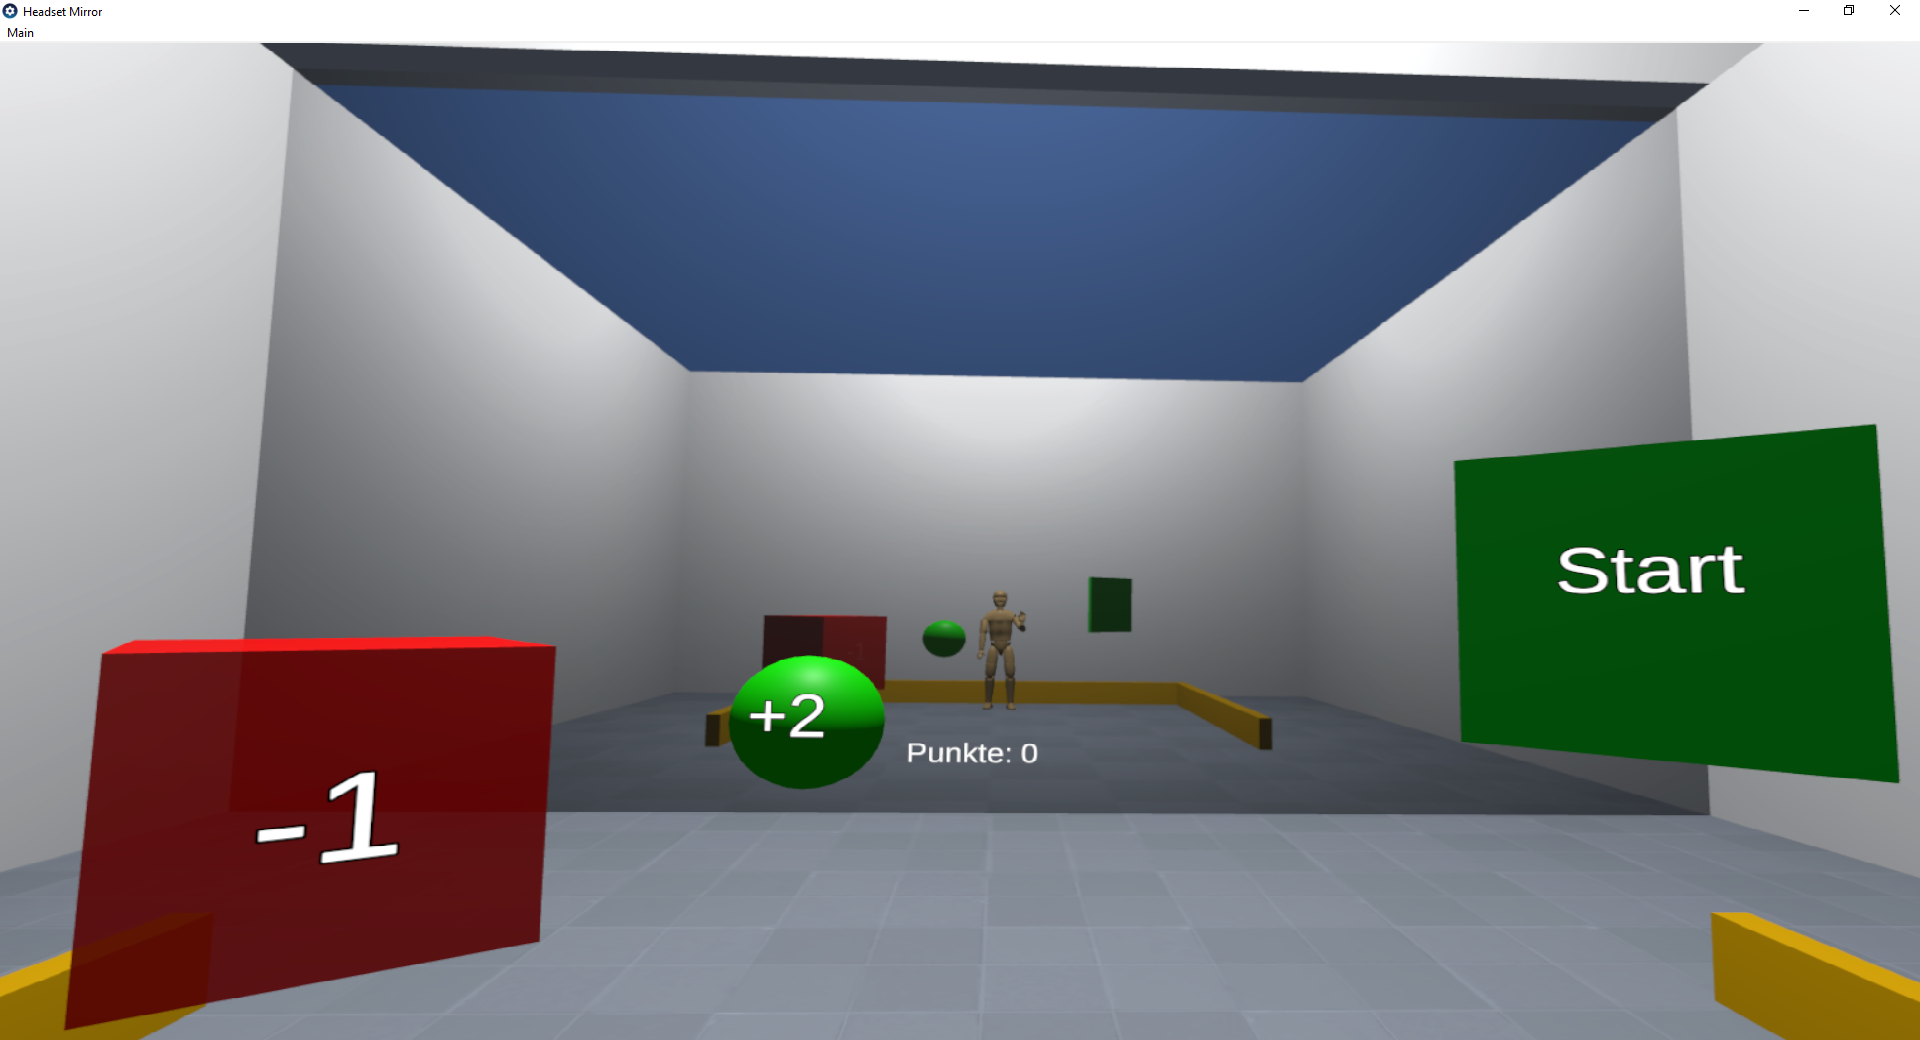
\includegraphics[width=\textwidth]{Bilder/Game/ingame.png}
  }
  \caption[Aktuelles Setup der Anwendung]{Sichtweise des Probanden wenn das Spiel gestartet wird.}
  \label{fig:povSetup}
\end{figure}

Die komplette Anwendung verzichtet auf Tasteneingaben des Benutzers, alle benötigten Eingaben passieren durch Berührung des Avatars mit den Objekten.
Sobald das Spiel gestartet wurde, bewegen sich von vorne aus dem Spiegel die Hazards und Collectibles in einem bestimmten Intervall und bewegen sich durch das begehbare Gebiet bis sie wieder aus der Rückwand verschwinden. Die Position der einzelnen Objekte wird vor dem Spiel zufällig innerhalb einem bestimmten Gebiet festgelegt. Zusätzlich können alle Objekte mit einer Wahrscheinlichkeit von 20 Prozent in der Luft schwebend statt auf dem Boden erscheinen. Dies soll den Spieler anregen, sich in gewissen Situationen zu ducken, um einem Hazard auszuweichen oder seine Hände zu bewegen um ein Collectible, welche über einem Hazard schwebt, einzusammeln. Während der gesamten Zeit wird dem Spieler seine Punktzahl angezeigt. Nachdem 40 Hazards und 20 Collectibles erschienen sind, ist das Spiel vorbei. Somit ist die höchste zu erreichende Punktzahl 40 und die niedrigste zu erreichende Punktzahl -40. Neben der gesamten Punktzahl werden bei Spielende die jeweils getroffenen Hazards und Collectibles angezeigt.
Sobald das Spiel beginnt, wird der Avatar ausgehend von der Position der HMD in alle Richtungen Skaliert. Das wirkt der unterschiedlichen Körpergröße bei verschiedenen Personen entgegen, da der Avatar bei kleineren Personen gebeugt steht oder bei größeren Personen den Boden nicht berührt.

mehr zum durchlauf



\section{Engine}
Die Anwendung wurde mithilfe der Unity Engine 2018.3.11f umgesetzt.
Unity bietet über den \textit{Assetstore} die Möglichkeit, Programme von Drittanbietern leicht in die eigene Anwendung zu integrieren. Die wichtigsten eingesetzten Assets für die Anwendung waren \textit{FinalIK} von rootmotion\cite{rootmotion} sowie SteamVR von Valve. FinalIK bietet vorgefertigte IK-Lösungen für eine Reihe an Anwendungsarten. Das im Experiment benutzte IK-Rig stammt von dem FinalIK Anwendungsbeispiel VRIK. Abbildung X zeigt die Standardkonfiguation der Knochen von VRIK. SteamVR bietet Grundfunktionalitäten für die HTC VIVE wie das Kamerarig und die Position der Controller. Die Textur für den Boden stammt ebenfalls aus SteamVR.


\section{Probleme}
Die größte Herausforderung während des Entwickeln als auch während des Versuchs war die große Anzahl an eingesetzter Hardware. Oft wurden scheinbar ohne Grund entweder die Tracker oder die Controller nicht erkannt oder konnten sich nicht mit SteamVR verbinden. Dies führte beim Versuch bei wenigen Testpersonen zu verminderter Immersion, da sie z.B. trotz Tracker ihren Ellbogen nicht bewegen konnten. 
Eine weitere Herausforderung war die Zuweisung der Tracker in Unity. Die SteamVR Anwendung besitzt kein benutzbares System, wie die Tracker konsistent dem gleichen Körperteil zugewiesen werden können. Letztendlich konnte ich im Code selbst die Zuweisung mithilfe der Herstellungsnummer der Tracker lösen.
Das Festmachen der Tracker am Körper bereitete ebenfalls viele Sorgen. Die Vive Tracker werden standardmäßig ohne Bänder zum Befestigen geliefert. Desweiteren gibt es keine offiziellen Bänder von Vive selbst. Meine Lösung beinhaltete beidseitiges Klettband mit Löchern für die von den Trackern benötigten Schrauben. Diese sind aber schwierig am Körper zu befestigen, wenn sie nicht rutschen sollen und sind anfällig dafür, dass die Tracker während der Anwendung rotieren.
 

\section{Versuchsdurchführung}
Der Versuch wurde im VR-Lab der Informatikfakultät der Hochschule Reutlingen durchgeführt. Der Raum bietet eine ca. drei mal sechs Meter große freie Fläche, die von zwei Vive tracking Kameras von einem Gerüst aus abgedeckt ist. Das Kabel des HTC VIVE HMDs ist lang genug, damit die ganze Fläche genutzt werden kann. Während des Versuchs wurde das Kabel von einer weiteren Person gehalten, damit während des Versuchs keine Stolpergefahr herrschte.

Von den 21 Probanden waren 14 männlich und 7 weiblich. Über 80 Prozent der Probanden hatten angegeben, dass bis zum Zeitpunkt der Versuchsdurchführung sehr wenig bis gar keine Erfahrung mit VR hatten. Bei den Probanden handelte es sich um eine Mischung aus Studenten der Fakultät Informatik sowie weiteren Personen, die nicht mit der Hochschule Reutlingen assoziiert sind. 
Eine Person gab an, leichte Übelkeit wären des Versuchs verspürt zu haben, brach den Versuch aber nicht ab. Jeder Teilnehmer hat den Versuch komplett beendet und alle Fragen beantwortet.

Bei einem Durchlauf in der Versuchsbedingung mit Trackern fiel einer der Controller aus, womit sich eine Hand des Avatars nicht mehr Bewegen lies. Der Durchlauf wurde nicht abgebrochen und die Antworten mit einem Kommentar in die Auswertung mit aufgenommen.




 
 
